We have identified the following persistent objects; APPOINTMENTS, LUCKYAPPOINTMENTS, USERS and NOFICATIONS. They are all saved by the server subsystem in a relational Database. When the user logs in, the Client synchronizes the users APPOINTMENTS, LUCKYAPPOINTMENTS and NOTIFICATIONS with the server, so that the Client subsystem is up to date with the changes, and the system can be used without connection. If local changes have not been saved to the server (probably due to loss of network connection), the system will synchronize next time a connection is established. This also means, that if a user has logged in to the system on a machine, it is possible to log in without connection later on, since the user-data is stored locally. There might be some problems with security or long periods without login, so we have yet to decide finer details of the synchronization between the Client and Server.

We considered saving persistent boundary objects locally, such as user preferences and last shown view, but we decided against it, since the client is supposed to be simple and intuitive, with ease of use and accessibility as declared design goals, making these boundary objects persistent, should not be necessary. 

\begin{figure}[ht]
\centering
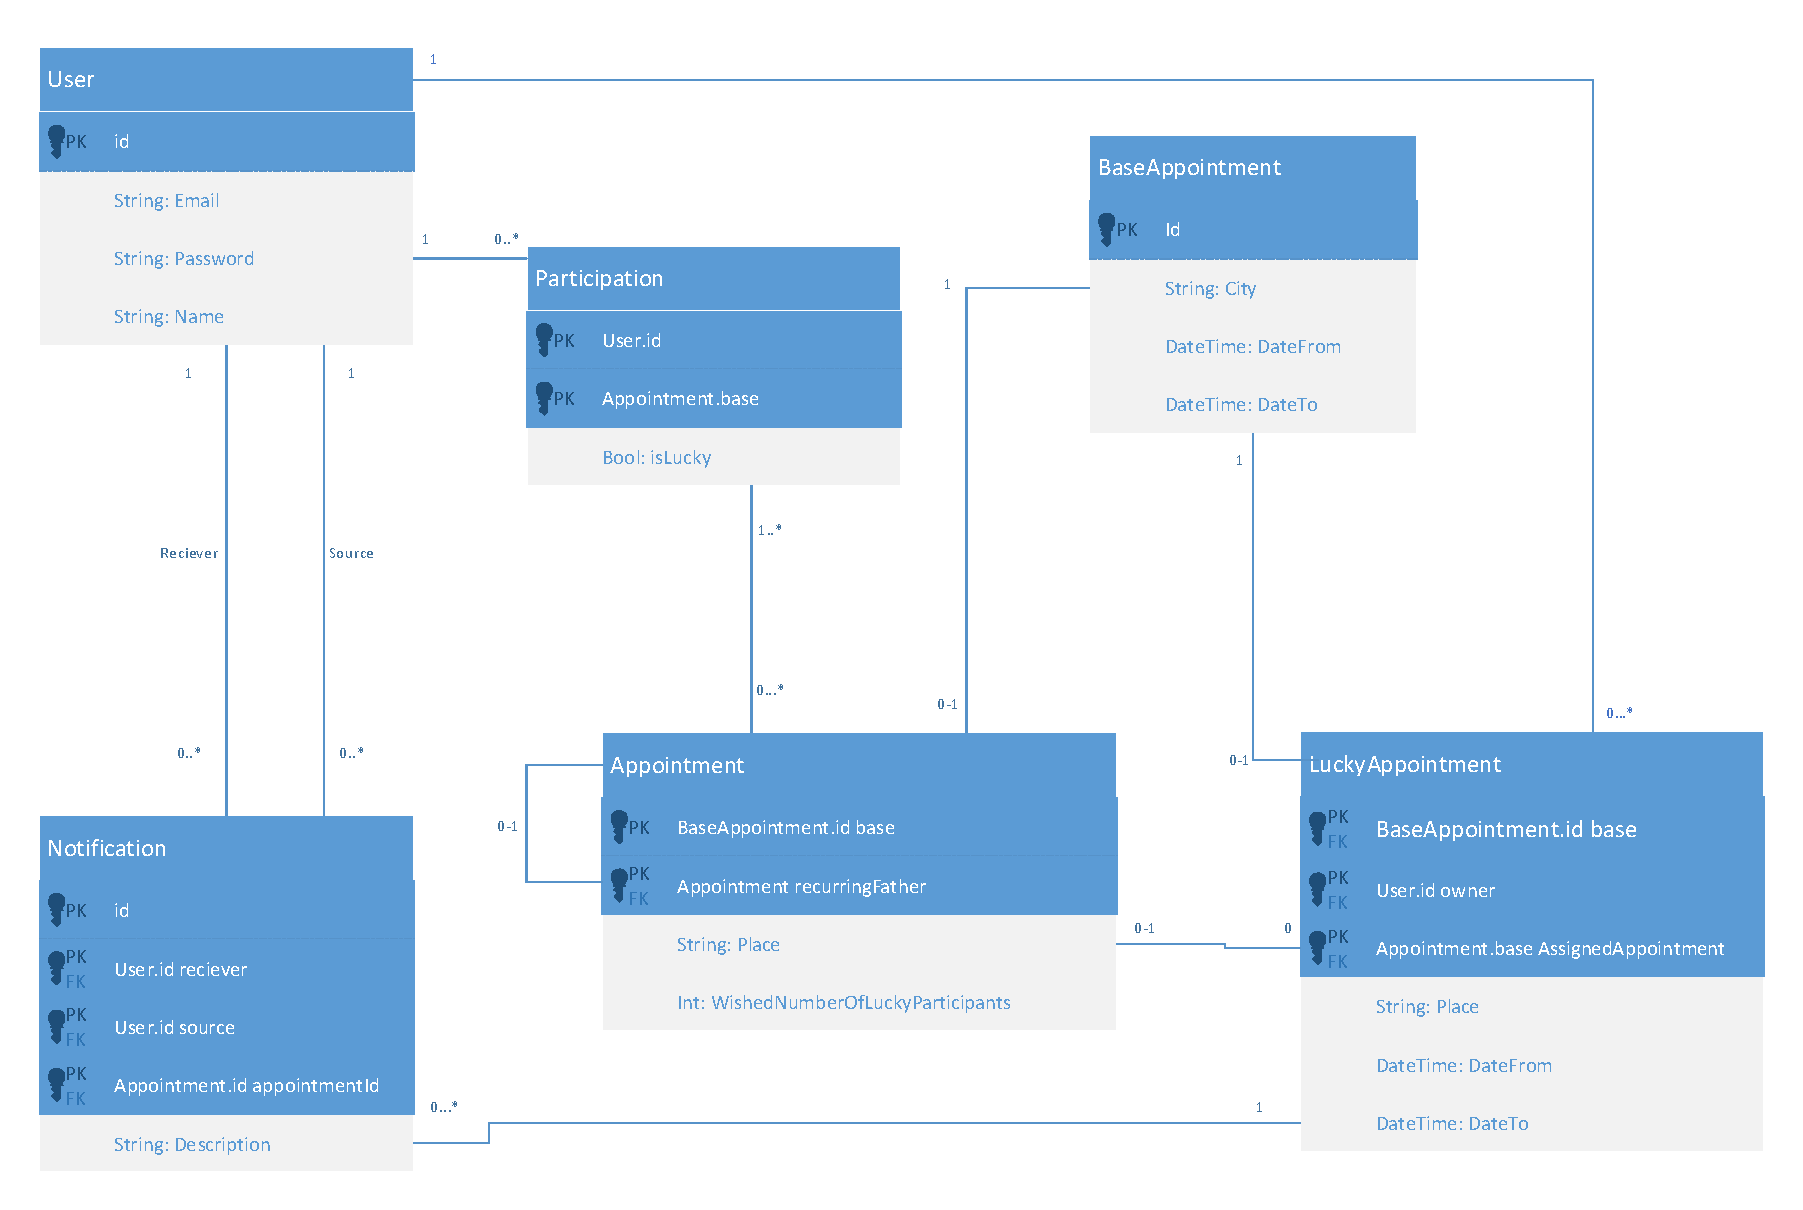
\includegraphics[scale=.35]{sections/db_mapping.pdf}
\caption{An entity/relation diagram of our database}
\end{figure}
